\documentclass{swfubeamer}

\title{Playing with a simple OS}
\author{CynYang}

\begin{document}

\frame{\titlepage}

\begin{frame}{Just for fun}
  \begin{center}
    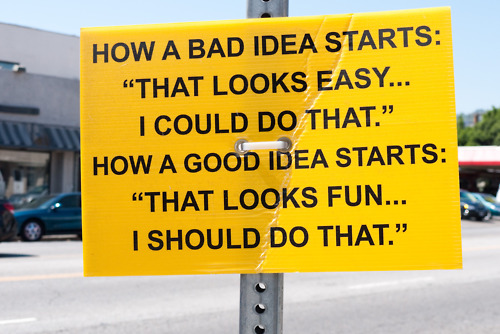
\includegraphics[width=.7\linewidth]{start}
  \end{center}
\end{frame}

\begin{frame}{Overview}
  \begin{center}
    \begin{minipage}{.2\linewidth}
      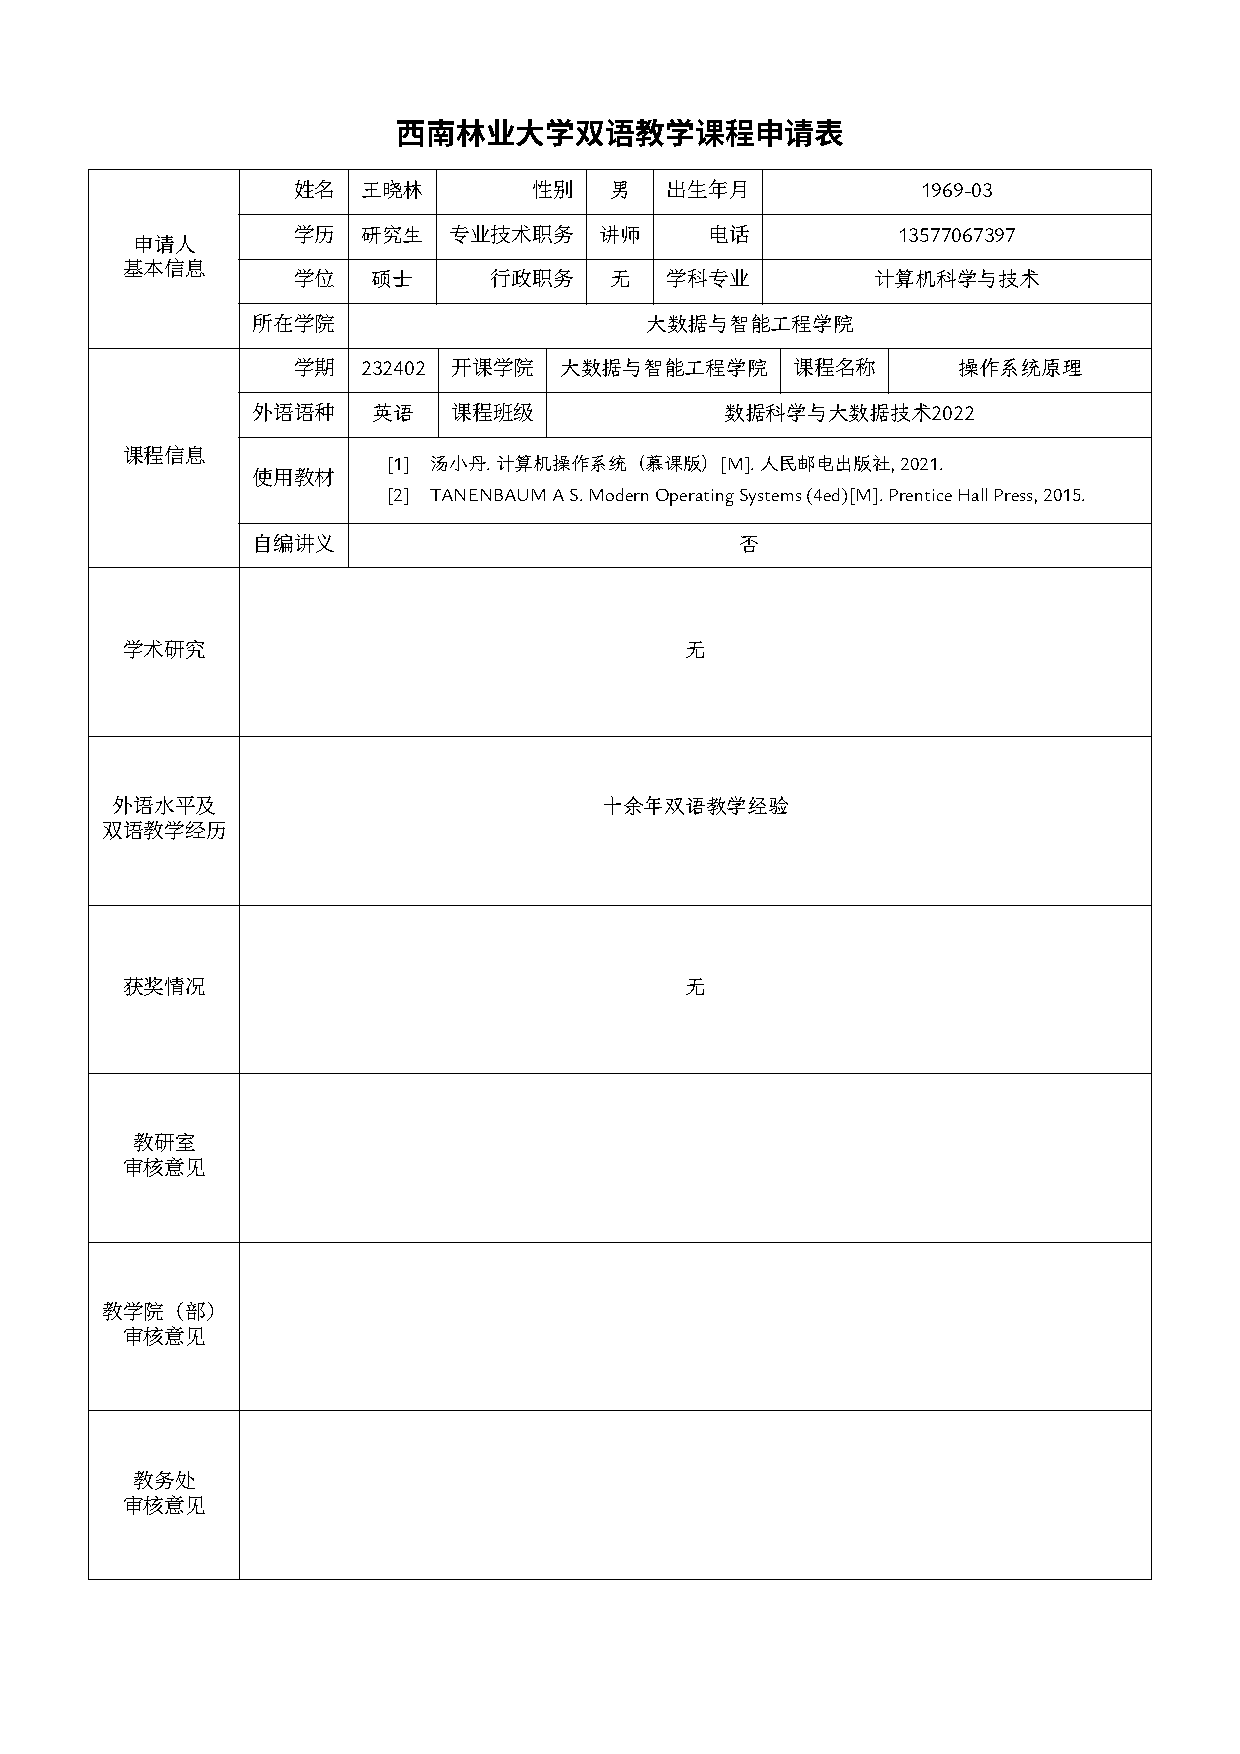
\includegraphics[width=\textwidth]{os}
    \end{minipage}\qquad\qquad
    \begin{minipage}{.45\linewidth}
      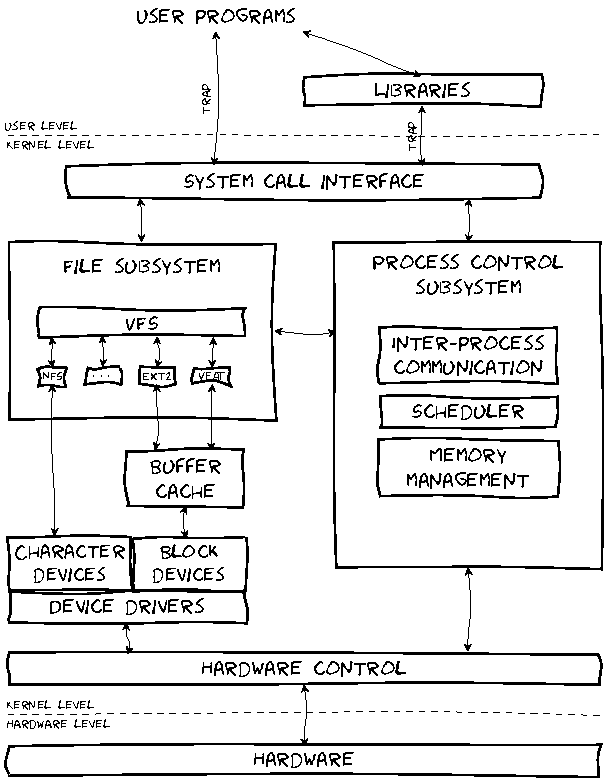
\includegraphics[width=\linewidth]{kernel-block}
    \end{minipage}
  \end{center}
\end{frame}

\begin{frame}{What I have done}
  \begin{itemize}
  \item Boot
  \item Screen output
  \item Keyboard input
  \item A user process
  \item A simple FS
  \item A few shell cmds
  \end{itemize}
\end{frame}

\begin{frame}
  \begin{center}
    Actions speak louder than words.\par\bigskip
    
    Let's do it\ldots
  \end{center}
\end{frame}


\end{document}

%%% Local Variables:
%%% mode: latex
%%% TeX-master: t
%%% End:
